\documentclass[envcountsect,10pt]{beamer}
    \usepackage[utf8]{inputenc}
    \usepackage[T1]{fontenc}
    \usepackage{pgfpages}
    \usepackage{url}
    \usepackage{bookmark}
    \usepackage{listings}
    \usepackage{xcolor}
    
\usetheme{Madrid}

% \setbeameroption{show notes}
% \setbeameroption{show notes on second screen=bottom}

\definecolor{darkgray}{rgb}{0.2,0.2,0.2}
\definecolor{darkgreen}{rgb}{0,0.6,0}

\lstdefinestyle{mystyle}{
    commentstyle=\color{darkgray},
    keywordstyle=\color{orange},
    stringstyle=\color{darkgreen},
    basicstyle=\ttfamily\footnotesize,
    breakatwhitespace=false,         
    breaklines=true,                 
    captionpos=b,                    
    keepspaces=true,                                    
    numbersep=5pt,                  
    showspaces=false,                
    showstringspaces=false,
    showtabs=false,                  
    tabsize=2
}

\lstset{style=mystyle}

\setbeamercolor{section title}{fg=white,bg=structure}

\setbeamertemplate{section page}
{
    \begingroup
        \centering
        \vskip1em\par
        \begin{beamercolorbox}[sep=12pt,center,shadow=true,rounded=true]{section title}
            \usebeamerfont{section title}\insertsection\par
        \end{beamercolorbox}
        \vskip0.5em\par
    \endgroup
}

\title{Functional Programming in Python}
\author{Jakub Dajczak}
\institute[]{Gdańsk University of Technology}
\date{Gdańsk, \the\year}

\begin{document}

\frame{\titlepage}

\begin{frame}
    \frametitle{Based on}

    \begin{center}
        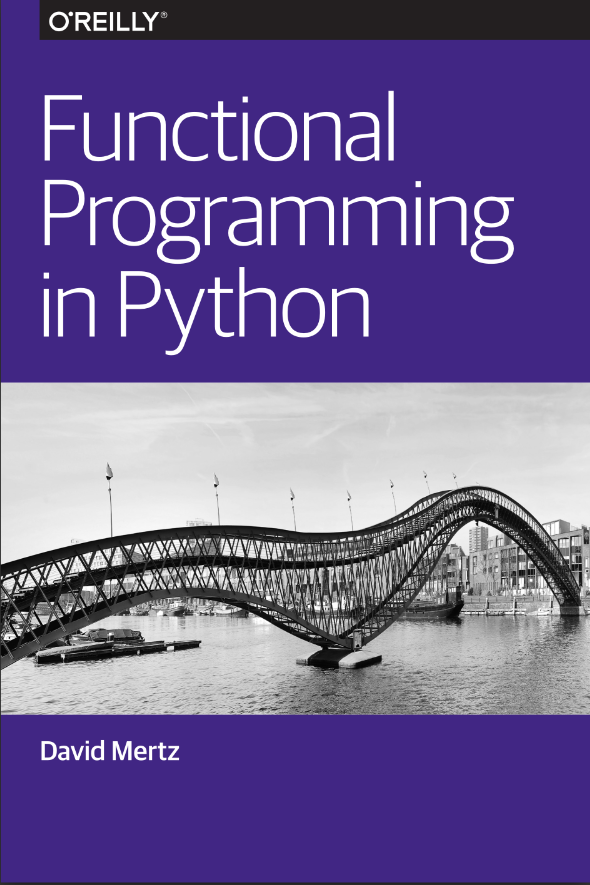
\includegraphics[width=0.4\textwidth]{book.png}
        
        \vspace{0.5em}
        \small{Functional Programming in Python}
    \end{center}
\end{frame}

\begin{frame}{Table of Contents}
    \centering
    \begin{columns}[t]
        \begin{column}{.4\textwidth}
            \tableofcontents[sections={1-3}]
        \end{column}
        \begin{column}{.4\textwidth}
            \tableofcontents[sections={4-5}]
        \end{column}
    \end{columns}
\end{frame}

\section{Typing}

\subsection{Type Hints}

\begin{frame}[fragile]
    \frametitle{Hints}

    Type hints improve code readability and help with static type checking.

    \begin{lstlisting}[language=Python]
>>> from typing import List, Dict, Tuple

>>> hello : str = "Hello, World!"
>>> names : List[str] = ["Alice", "Bob"]
>>> scores : Dict[str, int] = {"Alice": 100, "Bob": 95}
>>> vector : Tuple[int, int, int] = (1, 2, 3)
    \end{lstlisting}

    They can be also used in function definitions:

    \begin{lstlisting}
>>> def say_hello(names: List[str]) -> int:
...     for name in names:
...         print(f"Hello, {name}!")
...     return len(names)
    \end{lstlisting}

    Hints are stored in the \texttt{\_\_annotations\_\_} attribute of the function.

    \note{
        \LARGE
            \begin{itemize}
                \item Type hints are not enforced at runtime.
                \item User can technically ignore them and assign any value to a variable.
                \item Type checkers like mypy can be used to enforce type hints.
                \item It's a very debatable topic.
            \end{itemize}
    }

    \begin{lstlisting}
>>> say_hello.__annotations__
{'names': List[str], 'return': int}
    \end{lstlisting}
\end{frame}

\begin{frame}[fragile]
    \frametitle{Type Aliases}

    Type aliases can make complex type hints more readable and easier to manage.

    Using the \texttt{TypeAlias} from the \texttt{typing} module:

    \begin{lstlisting}[language=Python]
>>> from typing import TypeAlias, Tuple

>>> Vector3D : TypeAlias = Tuple[float, float, float]
    \end{lstlisting}

    Alternatively, using the \texttt{type} keyword:

    \begin{lstlisting}[language=Python]
>>> type Vector3D = Tuple[float, float, float]
    \end{lstlisting}

    The \texttt{Vector3D} alias represents a 3D vector as a tuple of three floats.

    \begin{lstlisting}[language=Python]
>>> v1 : Vector3D = (1.0, 2.4, 3.0)
>>> v2 : Vector3D = (4.0, 5.0, 6.1)
>>> add(v1, v2)
(5.0, 7.4, 9.1)
    \end{lstlisting}

    \note{
        \LARGE
            \begin{itemize}
                \item Type aliases can be used to simplify complex type hints.
            \end{itemize}
    }
\end{frame}

\subsection{Records}

\begin{frame}[fragile]
    \frametitle{\texttt{namedtuple}}

    \texttt{collections} module provides the \texttt{namedtuple} function to create simple, immutable record types.

    \begin{lstlisting}[language=Python]
>>> from collections import namedtuple
>>> Point = namedtuple('Point', ['x', 'y'])
>>> p = Point(1, 2)
    \end{lstlisting}

    Instances of \texttt{Point} have named fields and can be accessed by index or attribute.

    \begin{lstlisting}[language=Python]
>>> p.x
1
>>> p[1]
2
>>> p
Point(x=1, y=2)
    \end{lstlisting}

    \note{
        \LARGE
            \begin{itemize}
                \item As name suggests - it's a tuple with named fields.
                \item It's immutable by inheritance.
            \end{itemize}
    }
\end{frame}

\begin{frame}[fragile]
    \frametitle{\texttt{dataclass}}

    \texttt{dataclasses} module provides a \texttt{dataclass} decorator to create classes with less boilerplate.

    \begin{lstlisting}[language=Python]
>>> from dataclasses import dataclass

>>> @dataclass(frozen=True)
... class Point:
...     x: int
...     y: int
    \end{lstlisting}

    Instances of \texttt{Point} are mostly immutable by setting the \texttt{frozen} parameter to \texttt{True}.

    \begin{lstlisting}[language=Python]
>>> p = Point(1, 2)
>>> p.x
1
>>> p.y
2
>>> p
Point(x=1, y=2)
    \end{lstlisting}

    \note{
        \LARGE
            \begin{itemize}
                \item \texttt{dataclass} is a decorator that automatically generates special methods.
                \item Setting \texttt{frozen} to \texttt{True} makes instances mostly immutable.
                \item But using \texttt{setattr} method, it's possible to override this behavior.
            \end{itemize}
    }
\end{frame}

\section{(Avoiding) Flow Control}

\subsection{Comprehensions}

\begin{frame}[fragile]
    \frametitle{List Comprehensions}

    List comprehensions provide a concise way to create lists.

    Traditional \texttt{for} loop to filter and modify elements in a list:

    \begin{lstlisting}[language=Python]
>>> collection = []
>>> for datum in data_set:
...     if condition(datum):
...         collection.append(datum)
...     else:
...         new = modify(datum)
...         collection.append(new)
    \end{lstlisting}

    Using a list comprehension for the same task:

    \begin{lstlisting}[language=Python]
>>> collection = [datum if condition(datum) else modify(datum) for datum in data_set]
    \end{lstlisting}

    List comprehensions are more compact, readable, and often faster than traditional loops.

    \note{
        \LARGE
            \begin{itemize}
                \item It's pythonic way to create lists and other iterables.
                \item One of main python features.
                \item It's faster than traditional loops - definitely faster than insert
                \item Don't pack too much logic into a single line - readability is important.
            \end{itemize}
    }
\end{frame}

\begin{frame}[fragile]
    \frametitle{Other Comprehensions}

    Dictionary comprehension to create a mapping of indices to characters:
    \begin{lstlisting}[language=Python]
>>> {i:chr(65+i) for i in range(6)}
{0: 'A', 1: 'B', 2: 'C', 3: 'D', 4: 'E', 5: 'F'}
    \end{lstlisting}

    Set comprehension to create a set of characters:
    \begin{lstlisting}[language=Python]
>>> {chr(65+i) for i in range(6)}
{'A', 'B', 'C', 'D', 'E', 'F'}
    \end{lstlisting}

    Generator expression to lazily generate characters:
    \begin{lstlisting}[language=Python]
>>> (chr(65+i) for i in range(6))
<generator object <genexpr> at 0x7f8b1c1b3d60>
    \end{lstlisting}
\end{frame}

\begin{frame}[fragile]
    \frametitle{Generators}

    Generator functions declare a function that behaves like an iterator, allowing it to be used in a for loop. 
    Unlike lists, they are lazy and do not store all the values in memory.

    \begin{lstlisting}[language=Python]
>>> def count(n):
...     for i in range(n):
...         yield i

>>> c = count(5)
>>> c
<generator object count at 0x7f8b1c1b3d60>
>>> list(c)
[0, 1, 2, 3, 4]
    \end{lstlisting}

    \note{
        \LARGE
            \begin{itemize}
                \item They are lazy and can be infinite
            \end{itemize}
    }
\end{frame}

\subsection{Recursion}

\begin{frame}[fragile]
    \frametitle{Recursion}

    Python supports recursion, but it is not optimized for tail calls or deep recursion.
    It is best suited for problems that can be solved with a small number of recursive calls.

    \begin{lstlisting}[language=Python]
>>> def factorialI(N):
...     product = 1
...     while N >= 1:
...         product *= N
...         N -= 1
...     return product
    \end{lstlisting}

    \begin{lstlisting}[language=Python]
>>> def factorialR(N):
...     return 1 if N <= 1 else N * factorialR(N-1)
    \end{lstlisting}

    \note{
        \LARGE
            \begin{itemize}
                \item Type aliases can be used to simplify complex type hints.
            \end{itemize}
    }
\end{frame}

\section{Callables}

\subsection{Functions}

\begin{frame}[fragile]
    \frametitle{Pure Functions}

    Pure functions are functions where the output value is determined only by its input values, 
    without observable side effects.

    An impure function example:

    \begin{lstlisting}[language=Python]
>>> def print_and_add(x, y):
...     print(f"Adding {x} and {y}")
...     return x + y

>>> print_and_add(5, 3)
Adding 5 and 3
8
    \end{lstlisting}

    The function \texttt{print\_and\_add} is impure because it has a side effect (printing).

    \begin{lstlisting}[language=Python]
>>> def add(x, y):
...     return x + y

>>> add(5, 3)
8
    \end{lstlisting}

    \note{
        \LARGE
            \begin{itemize}
                \item Python also can easily access global variables by using \texttt{global} keyword.
                \item It's a good practice to avoid using global variables because it makes 
                functions less reusable and slows down code.
            \end{itemize}
    }
\end{frame}


\begin{frame}[fragile]
    \frametitle{Lambda Functions}

    Lambda functions are small anonymous functions defined with the \texttt{lambda} 
    keyword and they can be used wherever function objects are required.

    \begin{lstlisting}[language=Python]
>>> double = lambda x: x * 2
>>> double(3)
6
    \end{lstlisting}

    The name of a lambda function can be accessed or set using the \texttt{\_\_qualname\_\_} attribute.

    \begin{lstlisting}[language=Python]
>>> double.__qualname__
'lambda'
>>> len.__qualname__
'len'
    \end{lstlisting}

    \note{
        \LARGE
            \begin{itemize}
                \item Lambda functions are often used in functional programming.
                \item They are useful for short functions that are only used once.
            \end{itemize}
    }
\end{frame}

\begin{frame}[fragile]
    \frametitle{Closures}

    Python supports closures - functions that refer to variables from the scope in which they were defined.

    \begin{lstlisting}[language=Python]
>>> def f(x):
...     def g(y):
...         return x + y
...     return g

>>> add3 = f(3)
>>> add3(3)
6
>>> add3(5)
8
    \end{lstlisting}

    \note{
        \LARGE
            \begin{itemize}
                \item Closures are useful when you want to create a function that can be customized.
                \item They can be used as a factory.
            \end{itemize}
    }
\end{frame}

\begin{frame}[fragile]
    \frametitle{Unexpected Behavior}

    Closures can lead to unexpected behavior when the enclosed variable is mutable.

    \begin{lstlisting}[language=Python]
>>> adders = []
>>> for n in range(5):
...     adders.append(lambda m: m+n)
>>> [adder(10) for adder in adders]
[14, 14, 14, 14, 14]
>>> n = 10
>>> [adder(10) for adder in adders]
[20, 20, 20, 20, 20]
    \end{lstlisting}

    \note{
        \LARGE
            \begin{itemize}
                \item For loop creates n variable n that can be access outside this loop.
                \item Lambda function uses address of n variable, not the value.
                \item Of course n variable should not be available outside the loop.
            \end{itemize}
    }
\end{frame}

\begin{frame}[fragile]
    \frametitle{Unexpected Behavior}

    Fortunately, a small change brings behavior that probably better meets our goal:

    \begin{lstlisting}[language=Python]
>>> adders = []
>>> for n in range(5):
...     adders.append(lambda m, n=n: m+n)
>>> [adder(10) for adder in adders]
[10, 11, 12, 13, 14]
>>> n = 10
>>> [adder(10) for adder in adders]
[10, 11, 12, 13, 14]
>>> add4 = adders[4]
>>> add4(10, 100)  # Can override the bound value
110
    \end{lstlisting}

    \note{
        \LARGE
            \begin{itemize}
                \item By setting up a default value for n, we can avoid this problem.
                \item Setting a default value for saves n as value not as address.
                \item But now n can be overridden.
            \end{itemize}
    }
\end{frame}

\begin{frame}[fragile]
    \frametitle{Callable Instances}

    Callable instances can be created in Python by defining the \texttt{\_\_call\_\_} method in a class. 
    This approach is useful for creating objects that behave like functions.

    \begin{lstlisting}[language=Python]
>>> class Adder:
...     def __init__(self, x):
...         self.__x = x
...     def __call__(self, y):
...         return self.__x + y
    \end{lstlisting}

    \texttt{Adder} instances can be called with an argument to add a predefined value.

    \begin{lstlisting}[language=Python]
>>> add5 = Adder(5)
>>> add5(10)
15
>>> add5(3)
8
    \end{lstlisting}

    \note{
        \LARGE
            \begin{itemize}
                \item Python do not have private variables, but it has convention to use \texttt{\_\_} prefix.
                \item Of course we can change x to be easily changeable from outside.
                \item It's a good way to create a factory.
            \end{itemize}
    }
\end{frame}

\subsection{Pattern Matching}

\begin{frame}[fragile]
    \frametitle{\texttt{match} Statement}

    \begin{lstlisting}[language=Python]
>>> from dataclasses import dataclass
>>> from typing import Union
    \end{lstlisting}

Define dataclasses for shapes:

    \begin{lstlisting}[language=Python]
>>> @dataclass
... class Circle:
...     radius: float

>>> @dataclass
... class Rectangle:
...     width: float
...     height: float

>>> @dataclass
... class Triangle:
...     base: float
...     height: float
    \end{lstlisting}

A union type to represent all shapes:

    \begin{lstlisting}[language=Python]
>>> Shape = Union[Circle, Rectangle, Triangle]
    \end{lstlisting}

    \note{
        \LARGE
            \begin{itemize}
                \item Let's define shape classes.
                \item typing allows to define union types.
            \end{itemize}
    }
\end{frame}

\begin{frame}[fragile]
    \frametitle{\texttt{match} Statement}

    \texttt{match} can be used to define a function that describes a shape:

    \begin{lstlisting}[language=Python]
>>> def describe_shape(shape: Shape) -> str:
...     match shape:
...         case Circle(radius=r):
...             return f"A circle with radius {r}."
...         case Rectangle(width=w, height=h):
...             return f"A rectangle with width {w} and height {h}."
...         case Triangle(base=b, height=h):
...             return f"A triangle with base {b} and height {h}."
...         case _:
...             return "Not a valid shape."

>>> describe_shape(Circle(5))
'A circle with radius 5.'
>>> describe_shape(Rectangle(10, 20))
'A rectangle with width 10 and height 20.'
>>> describe_shape(Triangle(8, 6))
'A triangle with base 8 and height 6.'
>>> describe_shape(5)
'Not a valid shape.'
    \end{lstlisting}

    \note{
        \LARGE
            \begin{itemize}
                \item \texttt{match} statement is a new feature in Python 3.10.
                \item Before that people used \texttt{from multipledispatch import dispatch}
                \item @dispatch(int, int) - decorator for function
            \end{itemize}
    }
\end{frame}

\begin{frame}[fragile]
    \frametitle{\texttt{match} Statement for Lists}

    \texttt{match} statement can also be used to define a function that recursively sums a list of numbers:

    \begin{lstlisting}[language=Python]
>>> def sum_list(numbers):
...     match numbers:
...         case []:
...             return 0
...         case [head, *tail]:
...             return head + sum_list(tail)

>>> numbers = [1, 2, 3, 4, 5]
>>> sum_list(numbers)
15
>>> sum_list([])
0
    \end{lstlisting}

    \note{
        \LARGE
            \begin{itemize}
                \item Typical example we used on our course
                \item That allows us to use head, tail format
                \item We can also use single elements to use specified length
            \end{itemize}
    }
\end{frame}

\section{Higher-Order Functions}

\begin{frame}[fragile]
    \frametitle{Higher-Order Functions}

    In Python, functions are first-class objects, allowing them to be passed as arguments, 
    returned from other functions, and assigned to variables.

    \begin{lstlisting}[language=Python]
>>> def shout(text):
...     return text.upper()
...
>>> def whisper(text):
...     return text.lower()
...
>>> def greet(func):
...     return func("Hi, I am created by a function passed as an argument.")

>>> greet(shout)
'HI, I AM CREATED BY A FUNCTION PASSED AS AN ARGUMENT.'
>>> greet(whisper)
'hi, i am created by a function passed as an argument.'
    \end{lstlisting}

    \note{
        \LARGE
            \begin{itemize}
                \item first-class object - because in Python almost every thing is object
                \item shout and whisper could be lambas or pasted like text.lower
            \end{itemize}
    }

\end{frame}

\subsection{Decorators}

\begin{frame}[fragile]
    \frametitle{Function Composition}

    Using higher-order functions, it is possible to compose functions by chaining them together and creating a simple pipeline.

    \begin{lstlisting}[language=Python]
>>> def compose(*funcs):
...     def inner(data, funcs=funcs):
...         result = data
...         for f in reversed(funcs):
...             result = f(result)
...         return result
...     return inner

>>> times2 = lambda x: x*2
>>> minus3 = lambda x: x-3
>>> mod6 = lambda x: x%6
>>> f = compose(mod6, times2, minus3)
>>> all(f(i)==((i-3)*2)%6 for i in range(1000000))
True
    \end{lstlisting}

    \note{
        \LARGE
            \begin{itemize}
                \item It's a good way to create a pipeline.
                \item like using |> operator (forward pipe operator)
            \end{itemize}
    }
\end{frame}

\begin{frame}[fragile]
    \frametitle{Decorators}

    Decorators provide a convenient way to wrap additional behavior around 
    function calls, allowing reusable modifications like logging or validation.

    \begin{lstlisting}[language=Python]
>>> def decorator(func):
...     def wrapper():
...         print("Before calling the function.")
...         func()
...         print("After calling the function.")
...     return wrapper

>>> @decorator
... def greet():
...     print("Hello, World!")

>>> greet()
Before calling the function.
Hello, World!
After calling the function.
    \end{lstlisting}

    \note{
        \LARGE
            \begin{itemize}
                \item Decorators work as higher-order functions.
            \end{itemize}
    }
\end{frame}

\subsection{Useful Built-in Modules}

\begin{frame}[fragile]
    \frametitle{The \texttt{operator} Module}

    This module provides function equivalents of Python's built-in operators, 
    making it easier to pass them around or compose when building transformations alongside other utilities.

    \begin{lstlisting}[language=Python]
>>> import operator

>>> operator.add(1, 2) == 1 + 2
True
>>> operator.mul(3, 4) == 3 * 4
True
>>> operator.pow(2, 3) == 2 ** 3
True
    \end{lstlisting}

\end{frame}

\begin{frame}[fragile]
    \frametitle{The \texttt{itertools} Module}
    
    The \texttt{itertools} module provides iterable utilities such as 
    \texttt{accumulate} for partial computations or repeated applications of a function. 

    \begin{lstlisting}[language=Python]
>>> from operator import mul
>>> from itertools import accumulate, repeat
>>> data = [3, 4, 6, 2, 1, 9, 0, 7, 5, 8]

>>> list(accumulate(data, max))
[3, 4, 6, 6, 6, 9, 9, 9, 9, 9]

>>> list(accumulate(data, mul))
[3, 12, 72, 144, 144, 1296, 0, 0, 0, 0]

>>> update = lambda balance, payment: round(balance * 1.05) - payment
>>> list(accumulate(repeat(90, 10), update, initial=1000))
[1000, 960, 918, 874, 828, 779, 728, 674, 618, 559, 497]
    \end{lstlisting}

    \note{
        \LARGE
            \begin{itemize}
                \item accumulate - goes through iterable and returns partial results
                \item repeat - returns the same value multiple times
            \end{itemize}
    }
\end{frame}

\begin{frame}[fragile]
    \frametitle{The \texttt{functools} Module}

    The \texttt{functools} module provides higher-order functions that operate on other functions,
    making it easier to compose or partially apply functions.

    \begin{lstlisting}[language=Python]
>>> from functools import reduce
>>> from operator import mul

>>> def factorial(n):
...     return reduce(mul, range(1, n+1), 1)
    \end{lstlisting}

    \begin{lstlisting}[language=Python]
>>> from functools import partial

>>> def multiply(x, y):
...     return x * y

>>> double = partial(multiply, 2)
>>> double(4)
8
    \end{lstlisting}

    \note{
        \LARGE
            \begin{itemize}
                \item reduce - typical functional programming function
                \item partial - allows to create a new function with some arguments already set - curring
            \end{itemize}
    }

\end{frame}

\section{\texttt{returns} Library}

\subsection{Containers}

\begin{frame}[fragile]
    \frametitle{About \texttt{returns}}

    \begin{center}
        \textit{Make your functions return something meaningful, typed, and safe!}

        \vspace{2em}

        \url{https://github.com/dry-python/returns}
    \end{center}

    \note{
        \LARGE
            \begin{itemize}
                \item Randomly discovered it when searching about railroad programming in Python
                \item It nice way to use functional programming in Python 
            \end{itemize}
    }

\end{frame}

\begin{frame}[fragile]
    \frametitle{Maybe}

    \begin{lstlisting}[language=Python]
>>> @dataclass
... class Address(object):
...     street: Optional[str]

>>> @dataclass
... class User(object):
...     address: Optional[Address]

>>> @dataclass
... class Order(object):
...     user: Optional[User]

>>> def get_street_address(order: Order) -> Maybe[str]:
...     return Maybe.from_optional(order.user).bind_optional(
...         lambda user: user.address,
...     ).bind_optional(
...         lambda address: address.street,
...     )
    \end{lstlisting}

    \note{
        \LARGE
            \begin{itemize}
                \item Defined classes for user, address and order
                \item get\_street\_address function returns street address from order
                \item bind\_optional - binds a function that can return None and not Maybe
            \end{itemize}
    }
\end{frame}

\begin{frame}[fragile]
    \frametitle{Maybe}

    \begin{lstlisting}[language=Python]
>>> with_address = Order(User(Address('Some street')))
>>> empty_user = Order(None)
>>> empty_address = Order(User(None))
>>> empty_street = Order(User(Address(None)))

>>> get_street_address(with_address)
<Some: Some street>

>>> get_street_address(empty_user)
<Nothing>

>>> get_street_address(empty_address)
<Nothing>

>>> get_street_address(empty_street)
<Nothing>
    \end{lstlisting}

    \note{
        \LARGE
            \begin{itemize}
                \item As expected in railroad programming
                \item Maybe and other classes is immutable
                \item Like F\# Option type
            \end{itemize}
    }
\end{frame}

\begin{frame}[fragile]
    \frametitle{Maybe Decorator}

    \begin{lstlisting}[language=Python]
>>> from returns.maybe import maybe
        
>>> @maybe
... def number(num: int) -> Optional[int]:        
...     if num > 0:
...         return num
...     return None
        
>>> number(1)
<Some: 1>
>>> number(-1)
<Nothing>
    \end{lstlisting}

    \note{
        \LARGE
            \begin{itemize}
                \item Works like bind
                \item Converts Optional into Maybe Class
            \end{itemize}
    }
\end{frame}


\begin{frame}[fragile]
    \frametitle{Result}

    \begin{lstlisting}[language=Python]
>>> from returns.result import Result, Success, Failure

>>> def find_user(user_id: int) -> Result['User', str]:
...     user = User.objects.filter(id=user_id)
...     if user.exists():
...         return Success(user[0])
...     return Failure('User was not found')

>>> find_user(1)
<Success(User{id: 1, ...})>

>>> find_user(0)
<Failure('User was not found')>
    \end{lstlisting}

    \note{
        \LARGE
            \begin{itemize}
                \item Like F\# Result type
            \end{itemize}
    }
\end{frame}

\begin{frame}[fragile]
    \frametitle{Result Decorator}

    \begin{lstlisting}[language=Python]
>>> from returns.result import safe

>>> @safe  # Will convert type to: Callable[[int], Result[float, Exception]]
... def divide(number: int) -> float:
...     return number / number

>>> divide(1)
<Success(1.0)>

>>> divide(0)
<Failure: division by zero>
    \end{lstlisting}

    \note{
        \LARGE
            \begin{itemize}
                \item Catches errors and wraps them into Failure
                \item We can specify what errors we want to catch - like try except
            \end{itemize}
    }
\end{frame}

\subsection{Functions}

\begin{frame}[fragile]
    \frametitle{Pointfree}

    \begin{lstlisting}[language=Python]
>>> from returns.pointfree import map_

>>> def as_int(arg: str) -> int:
...     return ord(arg)

>>> container : Maybe[str] = Some('a')
>>> map_(as_int)(container) == container.map(as_int)
True
    \end{lstlisting}

    \note{
        \LARGE
            \begin{itemize}
                \item Way to use functions and not methods
                \item Allows map/bind non methods
            \end{itemize}
    }
\end{frame}

\begin{frame}[fragile]
    \frametitle{Trampolines}

    \note{Here's why we need trampolines: they allow to replicate tail call optimization by wrapping function calls into returns.trampolines.Trampoline objects, making recursion-based function always safe}

    \begin{lstlisting}[language=Python]
>>> from typing import Union, List
>>> from returns.trampolines import Trampoline, trampoline

>>> @trampoline
... def accumulate(numbers: List[int], acc: int = 0) -> Union[int, Trampoline[int]]:
...     if not numbers:
...         return acc
...     number = numbers.pop()
...     return Trampoline(accumulate, numbers, acc + number)

>>> accumulate([1, 2])
3
>>> accumulate([1, 2, 3])
6
    \end{lstlisting}

    \note{
        \LARGE
            \begin{itemize}
                \item Enables tail recursion for Python
            \end{itemize}
    }
\end{frame}

\begin{frame}[fragile]
    \frametitle{Fold}

    \begin{lstlisting}[language=Python]
>>> from typing import Callable
>>> from returns.maybe import Some
>>> from returns.iterables import Fold

>>> def sum_two(first: int) -> Callable[[int], int]:
...     return lambda second: first + second

>>> Fold.loop(
...     [Some(1), Some(2), Some(3)],
...     Some(10),
...     sum_two,
... )
<Some: 16>
    \end{lstlisting}
\end{frame}


\subsection{Pipelines}

\begin{frame}[fragile]
    \frametitle{Pipelines}

    \begin{lstlisting}[language=Python]
>>> from returns.result import Result, Success, Failure

>>> def regular_function(arg: int) -> float:
...     return float(arg)

>>> def returns_container(arg: float) -> Result[str, ValueError]:
...     if arg != 0:
...         return Success(str(arg))
...     return Failure(ValueError('Wrong arg'))

>>> def also_returns_container(arg: str) -> Result[str, ValueError]:
...     return Success(arg + '!')
    \end{lstlisting}
\end{frame}

\begin{frame}[fragile]
    \frametitle{\texttt{flow} function}

    \begin{lstlisting}[language=Python]
>>> from returns.pipeline import flow
>>> from returns.pointfree import bind

>>> flow(
...     1,
...     regular_function,
...     returns_container,
...     bind(also_returns_container),
... )
<Success: '1.0!'>

>>> flow(
...     0,
...     regular_function,
...     returns_container,
...     bind(also_returns_container),
... )
<Failure: Wrong arg>
    \end{lstlisting}
\end{frame}

\begin{frame}[fragile]
    \frametitle{\texttt{pipe} function}

    \begin{lstlisting}[language=Python]
>>> from returns.pipeline import pipe
>>> from returns.pointfree import bind

>>> transaction = pipe(
...     regular_function,
...     returns_container,
...     bind(also_returns_container),
... )
>>> transaction(1)
<Success: '1.0!'>
>>> transaction(0)
<Failure: Wrong arg>
    \end{lstlisting}
\end{frame}

\subsection{Interfaces}

\begin{frame}[fragile]
    \frametitle{Mappable}

    From the \texttt{returns} documentation:

    \textit{Something is considered mappable if we can map it using a function, generally map is a method that accepts a function.}
    \note{It is a functor.}

    \begin{lstlisting}[language=Python]
>>> from returns.maybe import Maybe, Some

>>> def can_be_mapped(string: str) -> str:
...     return string + '!'

>>> maybe_str: Maybe[str] = Some('example')

>>> assert maybe_str.map(can_be_mapped) == Some('example!')
    \end{lstlisting}
\end{frame}

\begin{frame}[fragile]
    \frametitle{Applicative}

    From the \texttt{returns} documentation:

    \textit{Something is considered applicative if it is a functor already and, moreover, we can apply another container to it and construct a new value with \texttt{.from\_value} method.}
    \note{It is a applicative.}

    \begin{lstlisting}[language=Python]
>>> from returns.maybe import Maybe, Some

>>> maybe_str = Maybe.from_value('example')

>>> maybe_func = Maybe.from_value(len)  # we use function as a value!

>>> assert maybe_str.apply(maybe_func) == Some(7)
    \end{lstlisting}
\end{frame}

\begin{frame}[fragile]
    \frametitle{Bindable}

    From the \texttt{returns} documentation:

    \textit{Bindable is something that we can bind with a function.}
    \note{It is a monad.}

    \begin{lstlisting}[language=Python]
>>> from returns.maybe import Nothing, Maybe, Some

>>> def bindable(string: str) -> Maybe[str]:
...     return Some(string + 'b')

>>> assert Some('a').bind(bindable) == Some('ab')
>>> assert Nothing.bind(bindable) == Nothing
    \end{lstlisting}
\end{frame}

\begin{frame}[allowframebreaks]
    \frametitle{Bibliography}

    \begin{itemize}
        \item \url{https://archive.org/details/functional-programming-python/mode/2up}
        \item \url{https://docs.python.org/3/howto/functional.html}
        \item \url{https://docs.python.org/3/library/typing.html}
        \item \url{https://github.com/sfermigier/awesome-functional-python?tab=readme-ov-file}
        \item \url{https://github.com/dry-python/returns}
        \item \url{https://docs.python.org/3/library/operator.html}
        \item \url{https://github.com/vickumar1981/functional_python/blob/master/functional-python.pdf}
        \item \url{https://noklam-data.medium.com/how-to-achieve-partial-immutability-with-python-dataclasses-or-attrs-0baa0d818898}
        \item \url{https://docs.python.org/3/library/itertools.html}
        \item \url{https://www.programiz.com/python-programming/closure}
        \item \url{https://peps.python.org/pep-0636/}
        \item \url{https://www.geeksforgeeks.org/python-match-case-statement/}
        \item \url{https://www.geeksforgeeks.org/python-lambda-anonymous-functions-filter-map-reduce/}
        \item \url{https://enauczanie.pg.edu.pl/moodle/course/view.php?id=41790}
        \item \url{https://www.geeksforgeeks.org/namedtuple-in-python/}
        \item \url{https://wiki.python.org/moin/Generators}
    \end{itemize}
\end{frame}

\begin{frame}
    \frametitle{Thank you!}

    \begin{center}
        \Huge
        Questions?
    \end{center}
\end{frame}

\end{document}